\section{Technische Dokumentation}
\subsection{Dokumentation der Storys}

\subsubsection{Der Benutzer möchte ein Fenster}

\begin{enumerate}
 \item Das Fenster ist sichtbar
 \item Das Fenster hat eine festgelegte größe
 \item Das Fenster kann verschoben werden
\end{enumerate}

\textbf{Storypoints:} 2 \\
\textbf{Bearbeitet von: } Fabian Zeller \\


\subsubsection{Der Benutzer möchte 3 Sektionen in dem Fenster}


\begin{enumerate}
 \item Die Sektionen sollen beschriftet sein
 \item Sektionen untereinander"
\end{enumerate}

\textbf{Storypoints:} 2 \\
\textbf{Bearbeitet von: } Fabian Zeller \\


\subsubsection{Der Benutzer möchte, dass in der unteren Sektion Klaviertasten angezeigt werden}

\begin{enumerate}
 \item Die Tasten haben 2 Farben (schwarz/weiß)
 \item Die Tasten können angeklickt werden
 \item Die Tasten sind wie auf einem Klavier angeordnet
\end{enumerate}

\textbf{Storypoints:} 5 \\
\textbf{Bearbeitet von: } Fabian Zeller \\


\subsubsection{Der Benutzer möchte mittels Tasten (Tastatur) einen Klavierton abspielen}

\begin{enumerate}
 \item Die Tasten spielen jeweils genanu einen Ton wenn sie geklickt werden
 \item Die Tasten können einen Ton halten
\end{enumerate}

\textbf{Storypoints:} 5 \\
\textbf{Bearbeitet von: } Emanuel Hubenschmid \\


\subsubsection{Der Programmierer arbeitet sich in Git-Hub ein}

\begin{enumerate}
 \item Das Git-Hub Repository kann von allen Programmierern benutzt werden
\end{enumerate}

\textbf{Storypoints:} 3 \\
\textbf{Bearbeitet von: } Fabian Zeller, Emanuel Hubenschmid \\

\subsubsection{Der Programmierer arbeitet sich in Javadocs ein}

\begin{enumerate}
 \item Die Javadoc-Seite soll alle wichtigen Informationen zu dem Programmquellcode enthalten
 \item Die Javadoc-Seite soll in der Dokumentation verlinkt werden
\end{enumerate}

\textbf{Storypoints:} 3 \\
\textbf{Bearbeitet von: } Fabian Zeller, Emanuel Hubenschmid \\


\subsubsection{Der Benutzer "möchte, dass die gespielte Taste hervorgehoben wird}

\begin{enumerate}
 \item Wenn eine Taste auf der Tastatur betätigt wird, färbt sich die entsprechende Taste auf dem 
Bildschirm
\end{enumerate}

\textbf{Storypoints:} 5 \\
\textbf{Bearbeitet von: } Fabian Zeller \\


\subsubsection{Der Benutzer möchte voreingestellte Samples auswählen können}

\begin{enumerate}
 \item Die Sample sollen die Tasten mit unterschiedlichen Tönen belegen
 \item Die voreingestellten Samples sollen Klaviertöne, Gitarrentöne, Basstöne und Schlagzeugtöne 
abspielen
\end{enumerate}

\textbf{Storypoints:} 5 \\
\textbf{Bearbeitet von: } Emanuel Hubenschmid \\


\subsubsection{Der Benutzer möchte mehrere Töne gleichzeitig spielen können}

\begin{enumerate}
 \item Die Töne sollen gleichzeitig abgespielt werden können
 \item Die Töne sollen nicht durch andere Töne unterbrochen werden
 \item Die Töne, die gleichzeitig angespielt wurden, sollen auch gleichzeitig abgespielt werden
 \item Die  anzahl der Töne die gleichzeitig gespielt werden können ist auf 3 beschränkt
\end{enumerate}

\textbf{Storypoints:} 5 \\
\textbf{Bearbeitet von: } Emanuel Hubenschmid \\


\subsubsection{Der Benutzer möchte, dass in der oberen Sektion Notenlinien angezeigt werden}

\begin{enumerate}
 \item Die Notenlinien bestehen aus fünf Linien
 \item Die Notenlinien beginnen mit einem Notenschlüssel
\end{enumerate}

\textbf{Storypoints:} 5 \\
\textbf{Bearbeitet von: } Fabian Zeller \\


\subsubsection{Der Benutzer möchte Notenlinien, auf denen Noten angezeigt und abgespeichert werden}

\begin{enumerate}
 \item Die Notenlinien speichern das Sample (pro Notenlinie genau ein Sample)
 \item Die Notenlinien sollen, mit den gespielten Noten, gespeichert werden können
 \item Noten speichern informationen
\end{enumerate}

\textbf{Storypoints:} 5 \\
\textbf{Bearbeitet von: } Fabian Zeller \\


\subsubsection{Der Benutzer möchte das gespielte Töne als Note angezeigt werden}

\begin{enumerate}
 \item Noten laufen die Notenlinie entlang
 \item Vorzeichen bei bestimmten Noten
\end{enumerate}

\textbf{Storypoints:} 8 \\
\textbf{Bearbeitet von: } Fabian Zeller \\


\subsubsection{Der Benutzer möchte das gespeicherte Notenlinien in einem externen Fenster aufgerufen 
werden können}

\begin{enumerate}
 \item Die Notenlinien  werden in einem externen Fenster geöffnet
 \item Die Notenlinien zeigen das Sample an indem sie aufgenommen wurden
\end{enumerate}

\textbf{Storypoints:} 5 \\
\textbf{Bearbeitet von: } Emanuel Hubenschmid \\


\subsubsection{Der Benutzer möchte gespeicherte Notenlinien abspielen}

\begin{enumerate}
 \item Die Notenlinien  können abgespielt, pausiert und gestoppt werden
 \item Die Notenlinien  können mit veränderbaren Tempo abgespielt werden
 \item Die Notenlinien  können mit Buttons abgespielt, pausiert und gestoppt werden
\end{enumerate}

\textbf{Storypoints:} 8 \\
\textbf{Bearbeitet von: } Emanuel Hubenschmid \\


\subsubsection{Der Benutzer möchte Noten, die auf den Notenlinien angezeigt und abgespeichert 
werden}

\begin{enumerate}
 \item Die Noten, die gespielt wurden, sollen auf den richtigen Notenlinien angezeigt werden
 \item Die Noten sollen die Tonhöhe speichern
 \item Die Noten sollen die Tonlänge speichern
 \item Die Noten sollen die Lautstärke speichern
\end{enumerate}

\textbf{Storypoints:} 8 \\
\textbf{Bearbeitet von: } Emanuel Hubenschmid \\


\subsubsection{Der Entwickler möchte eine Latex Dokumentation}

\begin{enumerate}
 \item Deckblatt
 \item Inhaltsverzeichniss
 \item Link auf Javadocs
 \item Quellen
\end{enumerate}

\textbf{Storypoints:} 5 \\
\textbf{Bearbeitet von: } Fabian Zeller, Emanuel Hubenschmid \\


\subsubsection{Der Benutzer möchte ein ToolBar-Menü}

\begin{enumerate}
 \item Die ToolBar enthält ein Hilfe-Menü
 \item Die ToolBar enthält ein Datei-Menü
 \item Das Datei-Menü enthält Steuerung zum managen von Aufnahmen und eigenen Samples ect.
\end{enumerate}

\textbf{Storypoints:} 3 \\
\textbf{Bearbeitet von: } Fabian Zeller, Emanuel Hubenschmid \\


\subsubsection{Der Benutzer möchte, dass in der Mittleren Sektion Buttons zur Steuerung angezeigt 
werden}

\begin{enumerate}
 \item Buttons und Felder zu Steuerung und Eingabe von Informationen zur Aufnahme von Tönen
 \item Tempo Dateiname müssen eingegeben werden
 \item Das Auswahlfeld der Samples ist ein Drop Down Menü
\end{enumerate}

\textbf{Storypoints:} 3 \\
\textbf{Bearbeitet von: } Emanuel Hubenschmid \\


\subsubsection{Der Benutzer möchte mit verschiedenen Button die aufgenommenen Noten abspielen 
lassen}

\begin{enumerate}
 \item Die Buttons spielen, sobald sie gedrückt werden, die gespeicherten Noten ab
 \item Die Buttons spielen die Noten mit einem einstellbaren Tempo ab
 \item Die Buttons können durch die F1 bis F12 Tasten betätigt werden
 \item Bei dem abspielen werden die Noten angezeigt
\end{enumerate}

\textbf{Storypoints:} 8 \\
\textbf{Bearbeitet von: } Emanuel Hubenschmid \\


\subsubsection{Der Benutzer möchte eingene Samples benutzen können}

\begin{enumerate}
 \item Die Samples sollen in eine Bibliothek geladen werden können
 \item Die Samples sollen vom Benutzer ausgewählt und abgespielt werden können
\end{enumerate}

\textbf{Storypoints:} 5 \\
\textbf{Bearbeitet von: } Emanuel Hubenschmid \\


\subsubsection{Der Benutzer möchte einen Projektordner erzeugen können}

\begin{enumerate}
 \item Der Projektordner enthält eine Sample- und einen Aufnahme-Ordner
\end{enumerate}

\textbf{Storypoints:} 8 \\
\textbf{Bearbeitet von: } Emanuel Hubenschmid \\


\subsubsection{Der Benutzer möchte das die Note einer Taste auf der Taste angezeigt wird}

\begin{enumerate}
 \item Sichtbare Note auf den Tasten
\end{enumerate}

\textbf{Storypoints:} 5 \\
\textbf{Bearbeitet von: } Fabian Zeller \\


\subsubsection{Der Benutzer möchte die Samples wechseln}

\begin{enumerate}
 \item Die Samples sollen mittels RadioButton ausgewählt werden können,
 \item Die RadioButton sollen für jede Taste das gleiche Sample auswählen
 \item Die Samples sollen mit Tasten gewächselt werden können"
\end{enumerate}

\textbf{Storypoints:} 5 \\
\textbf{Bearbeitet von: } Emanuel Hubenschmid \\


\newpage


\subsection{Klassendiagramme}
\subsection{Sequenzdiagramme}
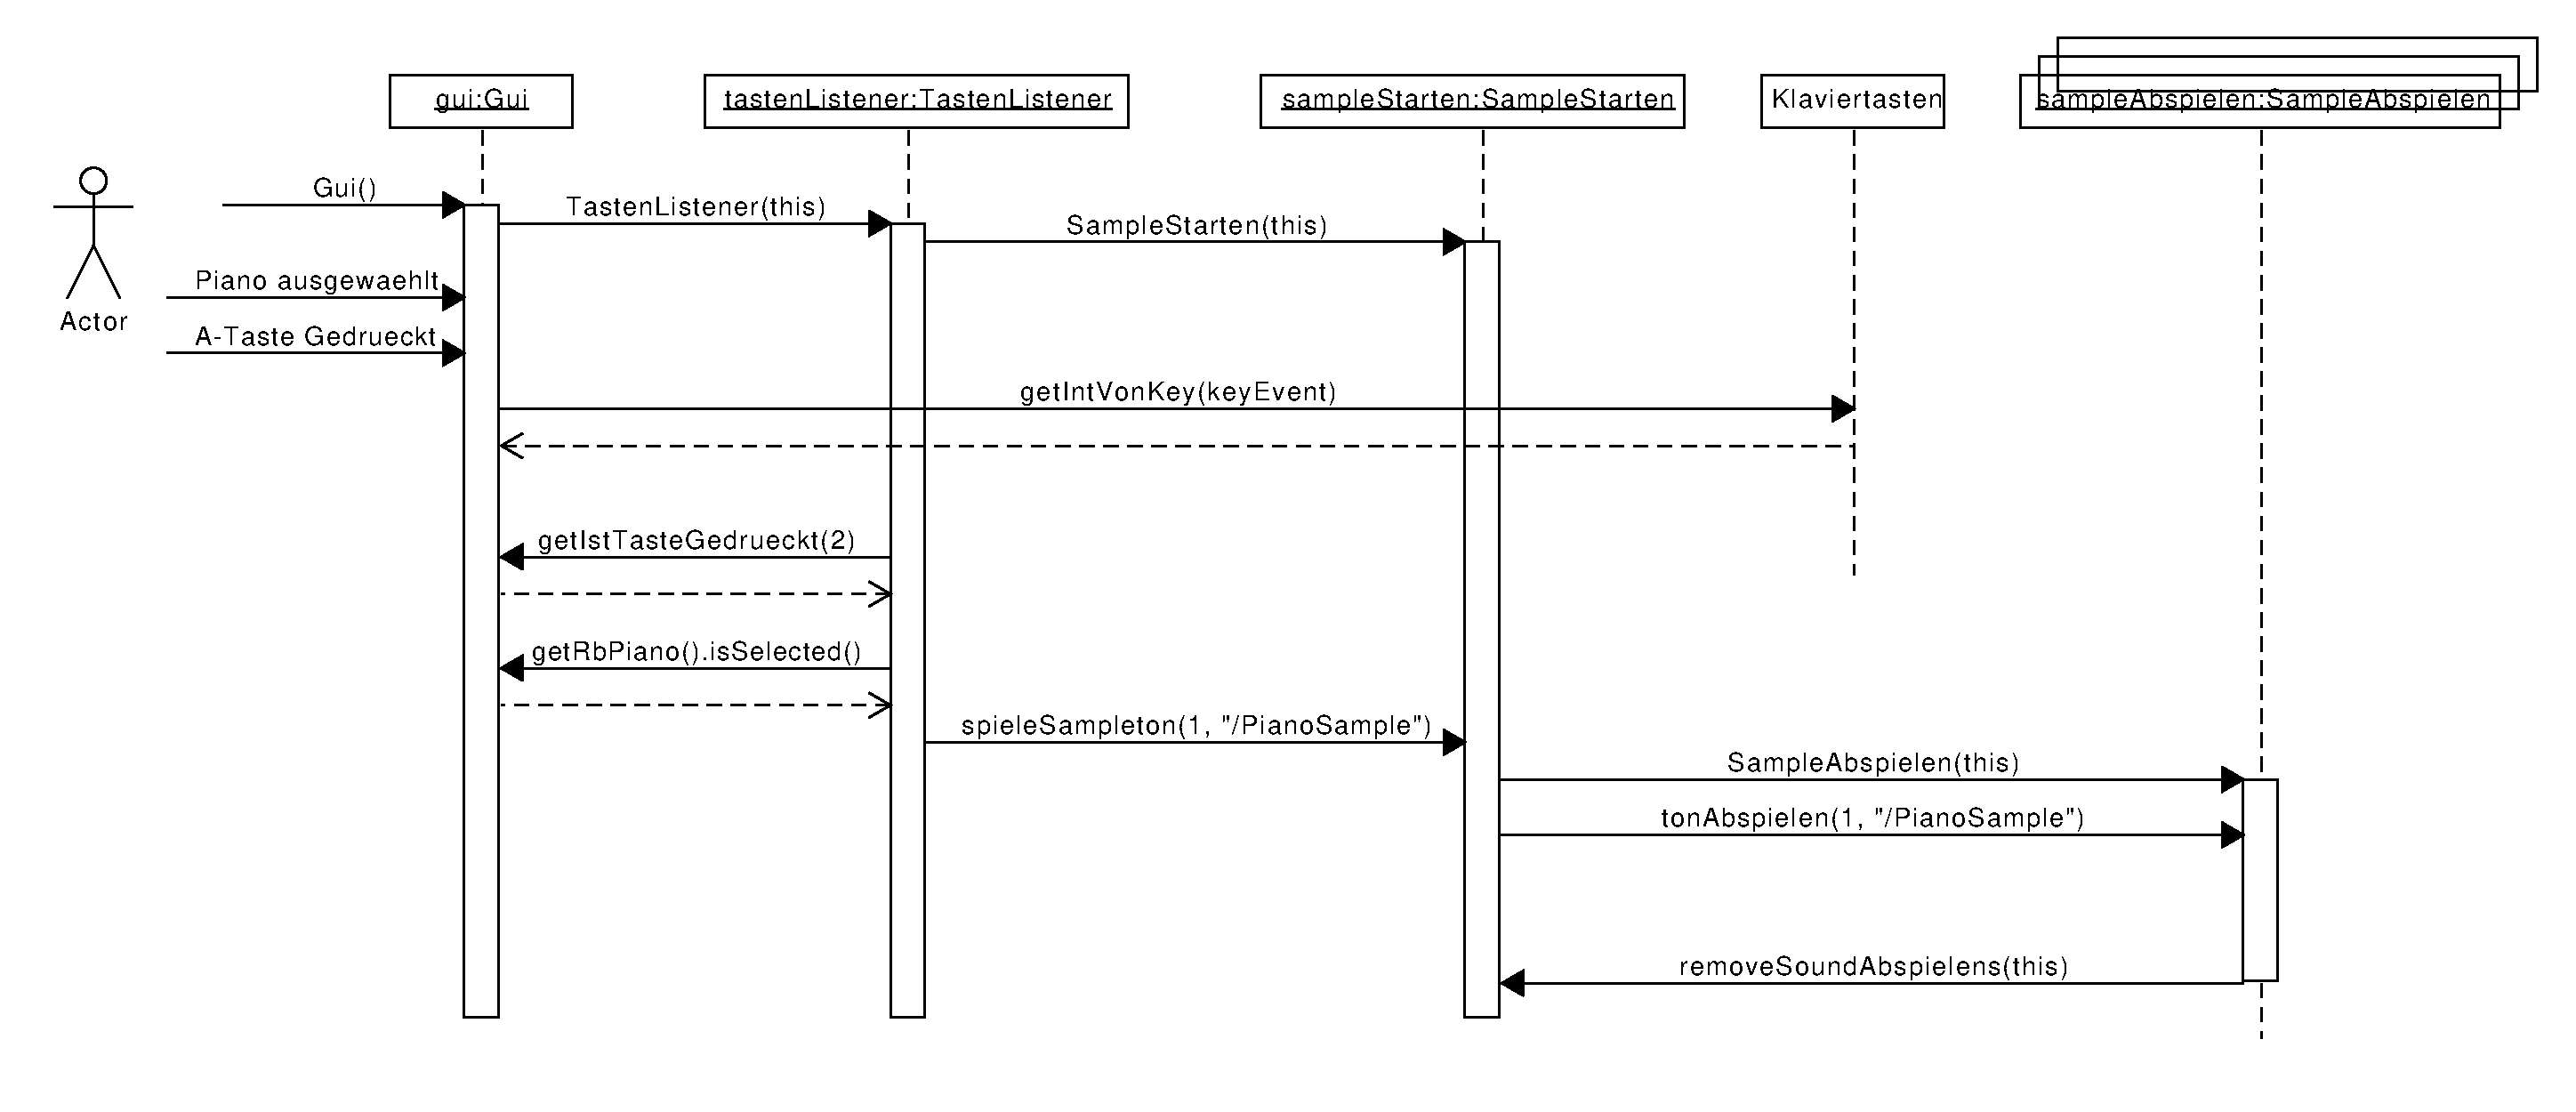
\includepdf{PDF/Klaviertaste_Gedrueckt.pdf}

\subsection{Beschreibung einiger Methoden}




Wir haben während des Projekts alle Methoden mithilfe von Javadocs dokumentiert. Unser komplettes 
Project ist also hier einsehbar: %Javadoc Zeug
\\

Einige größere Methoden werden wir in dieser Dokumentation allerdings etwas genauer beschreiben.

\subsection{Javadocs}
Der komplette Quelltext wurde mittels Javadocs auskommentiert. Hier kann nachgelesen werden, welche 
funktion die einzelnen Methoden erfüllen, sowie ihre Übergabe- und Rückgabeparameter, bzw. 
Exeptions  eingesehen werden.\\
Die komplette Javadocs Dokumentation kann hier geöffnet werden:\\
\url{./JavaDocs/index.html}